\documentclass[a4paper]{article}

\usepackage{amsfonts}
\usepackage{amssymb}
\usepackage{graphicx}
\usepackage{xcolor}
\usepackage{geometry}
\usepackage{titling}
\usepackage{caption}
\usepackage{algorithm}
\usepackage[noend]{algpseudocode}
\usepackage{listings}
\usepackage{xparse}
\usepackage{blindtext}
\usepackage{hyperref}
% \usepackage{xcolor}
\usepackage{mathtools}
\hypersetup{
    colorlinks=true,
    linkcolor=blue,
    filecolor=magenta,      
    urlcolor=cyan,
    pdftitle={Overleaf Example},
    pdfpagemode=FullScreen,
    }
\definecolor{darkBlue}{rgb}{0.1176, 0.14, 0.56}
\NewDocumentCommand{\codeword}{v}{%
\texttt{\textcolor{darkBlue}{#1}}%
}
\lstdefinestyle{sharpc}{language=[Sharp]C, frame=lr, rulecolor=\color{blue!80!black}}

\geometry{
   left=25.4mm,
   right=25.4mm,
   top=25.4mm,
   bottom=25.4mm,
}
\setlength{\droptitle}{-27mm}

\begin{document}
\author{Shridhar Thorat: n10817239}
\title{Assignment 1: CAB301}
\maketitle


\section{Test Plan}
Testing was done on an M1 Macbook Pro (MacOS Ventura 13.3.1 [22E261]). The test suite was designed using an MSTest project provided by Microsoft in the Visual Studio IDE on the {.}Net 7.0 framework.
\vspace{1.5mm}

\noindent
To ensure that all aspects of the software system cover functional, non-functional and boundary cases of methods, a comprehensive test plan was designed. The plan has been split into three sections that will delve deeper into what was tested each of the three ADTs and why.
\hyperlink{subsubsection.5.2.1}{appendix for CompareTo}.
\vspace{3mm}

\subsection{Movie ADT}

\subsubsection{CompareTo{(IMovie another)}}
The goal of \codeword{CompareTo} is to return -1 if this movie is less than another by dictionary order, 1 if it is greater, and 0 if it is the same.
\vspace{3mm}

\noindent
Since the movies need to be in dictionary order; the \codeword{String.CompareOrdinal} method was used. In order to test that the method worked properly, an array of movies with titles for each ASCII character from \codeword{space} to \codeword{~} was created. Each movie in the array was in descending order of ASCII value. 
\vspace{3mm}

\noindent
To test if $-1$ was outputted correctly, each \codeword{movie[i]} was \textit{compared to} each movie after it (\codeword{movie[i+1]}) where \codeword{i} ranged from $0$ to the length of the array of movies. It was expected that each comparison would output $-1$ since the movies were already arranged in descending order. This was called \codeword{CompareTo_Lower}.
\vspace{3mm}

\noindent
Similarly, to test if $1$ was outputted correctly, each \codeword{movie[i+1]} was \textit{compared to} each movie before it (\codeword{movie[i]}). Since movies were already arranged in descending order, a movie with a greater array index would have a greater ASCII value. Thus it was expected that each comparison would output $1$. This was called \codeword{CompareTo_Upper}
\vspace{3mm}

\noindent
To test if a movie titled compared to itself is $0$, each movie in the array was compared to itself. To ensure that the method didn't return $0$ because the movie had the same reference, a different array with the the same movies (but different objects) was also used. It was expected that each movie compared to a different movie instance, but with the same titles, would also output $0$. This was called \codeword{CompareTo_Same_with_same_object} and \codeword{CompareTo_Same_with_different_object} respectively. 
\vspace{1mm}

\noindent
From the below summary it can be seen that all tests passed and the method performend as required.These 4 tests can be found in the \hyperlink{subsubsection.5.2.1}{appendix for CompareTo}.
\vspace{3mm}

\noindent
\textbf{Unit testing summarisation}
\begin{figure}[H]
   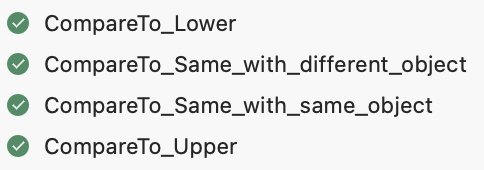
\includegraphics[height=2cm]{/Users/shridhar/Library/CloudStorage/OneDrive-QueenslandUniversityofTechnology/Bachelor of Mathematics and Information Technology/Year 4/CAB301 Algorithms/Assignment 2/Report/data/Summary-CompareTo.png}
\end{figure}

\subsubsection{ToString{()}}
ToString simply needed to output some of the properties of a movie. Hence there were only three tests; testing a movie will all properties defined, with only the movie title defined, and a movie with a null title (as this is the only property that can be set to null). The test data, results and testing code can be found in the \hyperlink{subsubsection.5.2.2}{appendix for ToString}. From the below summary it can be seen that all tests passed and the method performend as required.
\vspace{3mm}

\noindent
\textbf{Unit testing summarisation}
\begin{figure}[H]
   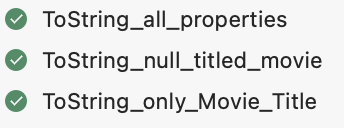
\includegraphics[height=1.8cm]{/Users/shridhar/Library/CloudStorage/OneDrive-QueenslandUniversityofTechnology/Bachelor of Mathematics and Information Technology/Year 4/CAB301 Algorithms/Assignment 2/Report/data/Summary-ToString.png}
\end{figure}

\subsection{MovieCollection ADT}
Since the methods implementated in the \codeword{MovieCollection} ADT all involve Movies and collecitons of Movies, they all used the same data; ofcourse, not all tests used all of the data. As the genre, classification, duration and available copies/total copies aren't relevant to the methods tested, they are kept constant for each different movie object. Additionally, \textit{single collection} refers to a collection with one movie and a \textit{large collection} is a collection with more than one movie.
\vspace{3mm}

\noindent
\textbf{Common Test Data}
\begin{figure}[H]
    \centering
    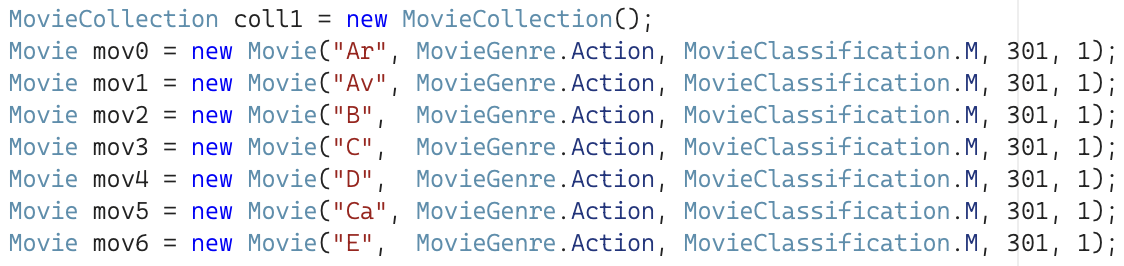
\includegraphics[height=3.2cm]{/Users/shridhar/Library/CloudStorage/OneDrive-QueenslandUniversityofTechnology/Bachelor of Mathematics and Information Technology/Year 4/CAB301 Algorithms/Assignment 2/Report/data/Common-data.png}
\end{figure}

\subsubsection{IsEmpty{()}}
\codeword{IsEmpty} was required to simply return \codeword{true} if a colection had no movies and \codeword{false} otherwise.

\begin{enumerate}
   \item \codeword{IsEmpty_True_empty_collection}: 
   
   \indent{
   Where the method returns \codeword{true} for an empty collection}
   \item \codeword{IsEmpty_True_after_deleting_single_collection}: 
   
   \indent{
   Where the method returns \codeword{true} after deleting the one movie in the collection.}
   \item \codeword{IsEmpty_True_after_deleting_large_collection}: 
   
   \indent{
      Where the method returns \codeword{true} after deleting all the movies in the collection.}
   \item \codeword{IsEmpty_False_single_collection}:
   
   \indent{
   Where the method returns \codeword{false} for a collection with one movie.
   }
   \item \codeword{IsEmpty_False_large_collection}: 
   
   \indent{Where the method returns \codeword{false} for a collection with lots of movie.}
\end{enumerate}
Technically testing the output to be \codeword{false} for a non-empty collection after all of its movie were deleted is not required since it uses another method; \codeword{Clear}. \codeword{Clear} was already tested to work correctly, hence it was used in the \codeword{IsEmpty} testing. Additionally, testing the output to be \codeword{true} when inserting multiple movies was also unnecessary since the number of movies will be greater than zero whether one or a million movies exist in a collection. However due to their trivial nature (and to prevent losing marks), they were still included. 

Additionally, for each of these tests, the post-condition that the the \codeword{count} property (read outside of the \textit{MovieCollection} class using the \codeword{Number} field) doesn't change before and after \codeword{IsEmpty} is called, was also checked.
\vspace{4mm}

\noindent
From the below summary it can be seen that all tests passed and the method performend as required. The test data, results and testing code can be found in the \hyperlink{subsubsection.5.3.1}{appendix for IsEmpty}. 
\vspace{1mm}

\noindent
\textbf{Unit testing summarisation}
\begin{figure}[H]
   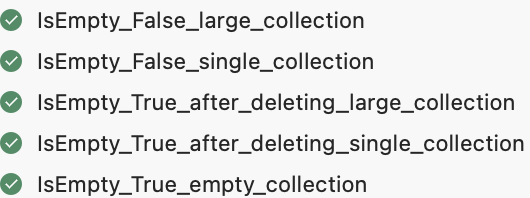
\includegraphics[height=2.3cm]{/Users/shridhar/Library/CloudStorage/OneDrive-QueenslandUniversityofTechnology/Bachelor of Mathematics and Information Technology/Year 4/CAB301 Algorithms/Assignment 2/Report/data/Summary-IsEmpty.png}
\end{figure}

\subsubsection{Insert{(IMovie movie)}}
The first test involved inserting a \codeword{root} to an empty collection and was done to ensure that the method correctly sets the \codeword{root} variable to the new movie. This is important as in this assignment a tree can only be traversed if the root is defined. This test was expected to return \codeword{true};
\vspace{2mm}

\noindent
The next two tests involed testing whether a \codeword{LChild} and \codeword{RChild} were inserted correctly and that the method returns \codeword{true}. Where a \codeword{RChild} must be greater than the root and the \codeword{LChild} is less than it in dictionary order. This is important to determine whether the collection is created correctly. It is worth mentioning, this test was done by checking whether the \codeword{Insert} method writes \codeword{`movie is a RChild'} or \codeword{`movie is a LChild'} into a line in the Visual Studio `console' for a given \codeword{movie} parameter that is inserted successfully.
\vspace{2mm}

\noindent
Next, it was tested whether trying to insert a movie that already exists in a single collection returns \codeword{false} and the movie is not inserted (by checking if \codeword{Number} is invariant).
\vspace{2mm}

\noindent
Lastly, as a sanity check, it was tested whether inserting multiple movies all outputted true. It is worth noting that testing insertion of multiple movies is not required. This is because inserting a movie into a Binary Search Tree is never done between existing movie but only as leaves. For example, if collection has a \codeword{root} as `Batman' and it's \codeword{RChild} was `Dungeons and Dragons'. Then inserting `Cars' wouldn't make it the new \codeword{RChild} of `Batman' but the \codeword{LChild} of `Dungeons and Dragons'. 
\vspace{2mm}

\noindent
Additionally, for each of test, the post-condition was tested --- that the \codeword{Number} of movies of increments by 1 if \codeword{Insert} is successful (returns \codeword{true}) and doesn't change if it is unsuccessfull (returns \codeword{false}).
\vspace{2mm}

\noindent
From the below summary it can be seen that all tests passed and the method performend as required.
\vspace{4mm}

\noindent
These tests were names intuitively are summarised below. Test data, results and testing code can be found in the \hyperlink{subsubsection.5.3.2}{appendix for Insert}.
\vspace{1mm}

\noindent
\textbf{Unit testing summarisation}
\begin{figure}[H]
   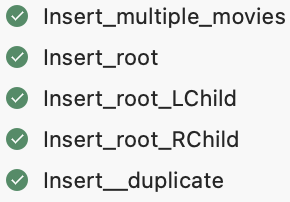
\includegraphics[height=2.8cm]{/Users/shridhar/Library/CloudStorage/OneDrive-QueenslandUniversityofTechnology/Bachelor of Mathematics and Information Technology/Year 4/CAB301 Algorithms/Assignment 2/Report/data/Summary-Insert.png}
\end{figure}

\subsubsection{ToArray{()}}
The \codeword{ToArray} method simply returns an \codeword{IMovie} array containing \codeword{Movie} objects, sorted in dictionary order. Thus, testing involved checking if the sorting was correct for a \textit{single} collection and \textit{large} collection, as well as for an empty collection; in which case the output was expected to be an empty \codeword{IMovie} array (i.e. \codeword{new IMovie[0]}). 
\vspace{1mm}

\noindent
The below summary shows these three all passed. Test data, results and code can be found in the \hyperlink{subsubsection.5.3.3}{appendix for ToArray}.
\vspace{2mm}

\noindent
\textbf{Unit testing summarisation}
\begin{figure}[H]
   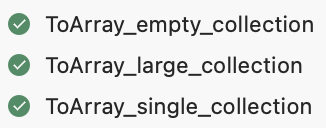
\includegraphics[height=1.8cm]{/Users/shridhar/Library/CloudStorage/OneDrive-QueenslandUniversityofTechnology/Bachelor of Mathematics and Information Technology/Year 4/CAB301 Algorithms/Assignment 2/Report/data/Summary-ToArray.png}
\end{figure}

\subsubsection{Search{(string title)}}
The \codeword{Search} method was designed to return a reference to an \codeword{IMovie} object if the movie is in `\codeword{this}' movie collection and \codeword{null} otherwise. A number of tests were designed to ensure these conditions were met.
\vspace{3mm}

\noindent
To test if the correct ouput was \codeword{null}, the method was tested against an empty collection with a \codeword{non-null} \textbf{title}, a \textit{single} and \textit{large} collection with a \codeword{null} \textbf{title} as well as a \textbf{title}; that is not in either collection. 
\vspace{3mm}

\noindent
To test if the correct output was a reference, the method was tested using a movie \textbf{title} known to exist in a \textit{single} and a \textit{large} collection.
\vspace{1mm}

\noindent
Of course, the post-condition that the \codeword{Number} of movies remains unchanged and the object passed is a reference rather tha independent copy, was also checked for each of the 7 tests. As summarised below, each of these tests passed. Test data, results and code can be found in the \hyperlink{subsubsection.5.3.4}{appendix for Search}.
\vspace{2mm}

\noindent
\textbf{Unit testing summarisation}
\begin{figure}[H]
   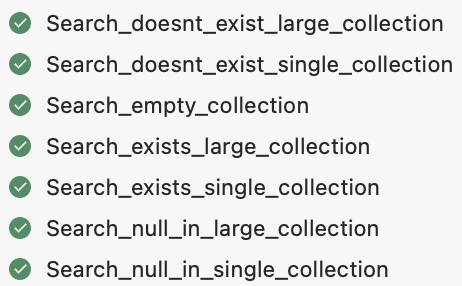
\includegraphics[height=3.5cm]{/Users/shridhar/Library/CloudStorage/OneDrive-QueenslandUniversityofTechnology/Bachelor of Mathematics and Information Technology/Year 4/CAB301 Algorithms/Assignment 2/Report/data/Summary-Search.png}
\end{figure}

\subsubsection{Delete{(IMovie movie)}}
If the parameter \codeword{movie} is in the collection, the \codeword{Delete} method would remove it and return \codeword{true} and decrement the \codeword{Number} value by 1 and return \codeword{false} otherwise while also leaving the \codeword{Number} parameter unchanged.
\vspace{1mm}

Additionally, it was assumed that when deleting a node (movie) that isn't a leaf and has two children, it would be replaced by the \textit{right most node in the left sub-tree} of that node; similar to lecture material. It is worth mentioning that \codeword{ToArray} was used to test if the structure of the collection was preserved.
\vspace{2mm}


\noindent
For the tests where the method returned \codeword{false} the post-condition that the \codeword{Number} of movies is unchanged ($oldNumber = newNumber$) and that the collection remains unchanged (\codeword{ToArray} is the same before and after false deletion) was checked.
\vspace{1.5mm}

For the tests where \codeword{Delete} was \codeword{true}, the post-condition that the deleted movie could no longer be found in the collection (using \codeword{Search}); signifying that it was correctly set to null and no longer exists was checked. The other post-condition that \codeword{Number} decrements (i.e $oldNumber=newNumber+1$) was checked.

\noindent
The 13 tests can be summarised below. Note that for \textbf{9} to \textbf{13}, the deleted \codeword{node} is not a leaf or a root for the collection. 
\begin{enumerate}
   \item \codeword{Delete_node_not_in_single_collection}
   
   \indent{Where the method returns \codeword{false} when the movie is not in a collection with one movie.}
   \item \codeword{Delete_node_not_in_large_collection}
   
   \indent{Where the method returns \codeword{false} when the movie is not in a collection with multiple movies}
   \item \codeword{Delete_node_not_in_empty_collection.}
   
   \indent{Where the method returns \codeword{false} when the movie is not in an empty collection.}
   \item \codeword{Delete_null_node_in_single_collection}
   
   \indent{Where the method returns \codeword{false} when the movie is \codeword{null} for a collection with only one movie.}
   \item \codeword{Delete_root_single_collection}
   
   \indent{Where the method returns \codeword{true} when the movie is deleted from a collection with only one movie.}
   \item \codeword{Delete_root_has_only_LChild}
   
   \indent{Where the method returns \codeword{true} when the movie is deleted from a collection with only a \codeword{root} and its \codeword{LChild}. The new root is the deleted node's \codeword{LChild}; confirmed by checking if \codeword{Search}-ing for \codeword{LChild} is \codeword{true} since \codeword{Search} traverses the collection starting at the \codeword{root}.}
   \item \codeword{Delete_root_has_only_RChild}
   
   \indent{Where the method returns \codeword{true} when the movie is deleted from a collection with only a \codeword{root} and its \codeword{RChild}. The new root is the deleted node's \codeword{RChild}; confirmed by checking if \codeword{Search}-ing for \codeword{LChild} is \codeword{true} since \codeword{Search} traverses the collection starting at the \codeword{root}.}
   \item \codeword{Delete_root_has_LChild_and_RChild_as_leaves}
   
   \noindent{Where the method returns \codeword{true} when the \codeword{root} is deleted from a collection with a \codeword{root} having  \textbf{both} a \codeword{LChild} \textbf{and} \codeword{RChild}. The new root becomes the deleted node's \codeword{LChild}; confirmed by checking if \codeword{coll1.ToArray} is confirmed to be in dictionary order. Since \codeword{ToArray} uses an $In-Order~traversal~method$, if the node was replaced by its \codeword{RChild} the order would then be \textit{D, B} rather than \textit{B, D} which would result from \codeword{LChild} becoming the root}.
   \item \codeword{Delete_node_has_only_LChild_leaf}
   
   \noindent{Where the method returns \codeword{true} when a node that only has a \codeword{LChild} leaf, is deleted. \codeword{LChild} is confirmed to replace it by checking if the \codeword{coll1.ToArray} method doesn't contains a \codeword{null} value, since if the non-existent \codeword{RChild} replaces the node, the collection will have a movie with a \codeword{null} title.}
   \item \codeword{Delete_node_has_only_RChild_leaf}
   
   \noindent{Where the method returns \codeword{true} when a node that only has a \codeword{RChild} leaf, is deleted. \codeword{RChild} is confirmed to replace it by checking if the \codeword{coll1.ToArray} method doesn't contains a \codeword{null} value, since if the non-existent \codeword{LChild} replaces the node, the collection will have a movie with a \codeword{null} title. }
   \item \codeword{Delete_node_has_LChild_and_RChild_as_leaves}
   
   \noindent{Where the method returns \codeword{true} when a node that has a \codeword{RChild} leaf and \codeword{LChild} leaf, is deleted. \codeword{LChild} is confirmed to replace it by checking if the \codeword{coll1.ToArray} method is in dictionary order. Since \codeword{ToArray} uses a $In-Order~traversal~method$, if the node was replaced by its \codeword{RChild} the order would then be \textit{Av, D, B} which is incorrect. And if it was replaced by \codeword{LChild} the order would be \textit{Av, B, D}, which is correct.}
   \item \codeword{Delete_node_has_LChild_with_LeftSkewedtree_and_RChild_as_leaf}
   
   \noindent{Where the method returns \codeword{true} when a node that has a \codeword{RChild} leaf and and a \codeword{LChild} with a left-skewed sub-tree, is deleted, and replaced by the immediate \codeword{LChild}. The replacement is checked to be correct by confirming that \codeword{coll1.ToArray} is in dictionary order. Since \codeword{ToArray} uses an $In-Order~traversal~method$, if the node was replaced by its non-immediate \codeword{LChild}; \codeword{Av}, the order would then be \textit{Ar, B, Av, Ca}--- which is incorrect, rather than \textit{Ar, Av, B, Ca} which would result from the immediate \codeword{LChild} being the replacement.}
   \item \codeword{Delete_node_has_LChild_with_RightSkewedtree_and_RChild_as_leaf}
   
   \noindent{Where the method returns \codeword{true} when a node that has a \codeword{RChild} leaf and and a \codeword{LChild} with a right-skewed sub-tree, is deleted, and replaced by the \textit{right most node in its left sub-tree}. The replacement is checked to be correct by confirming that \codeword{coll1.ToArray} is in dictionary order. Since \codeword{ToArray} uses an $In-Order~traversal~method$, if the node was replaced by its immediate \codeword{LChild}; \codeword{Ar}, the order would then be \textit{B, Av, Ar, D, E}--- which is incorrect, rather than \textit{Av, Ar, B, D, E} which would result from the \textit{right most node in its left sub-tree}; \codeword{B}, being the replacement.}
\end{enumerate}
\noindent


\noindent
As summarised below, each of these tests passed and the method was confirmed to perform as required. Test data, results and code can be found in the \hyperlink{subsubsection.5.3.5}{appendix for Delete}.
\vspace{2mm}

\noindent
\textbf{Unit testing summarisation}
\begin{figure}[H]
   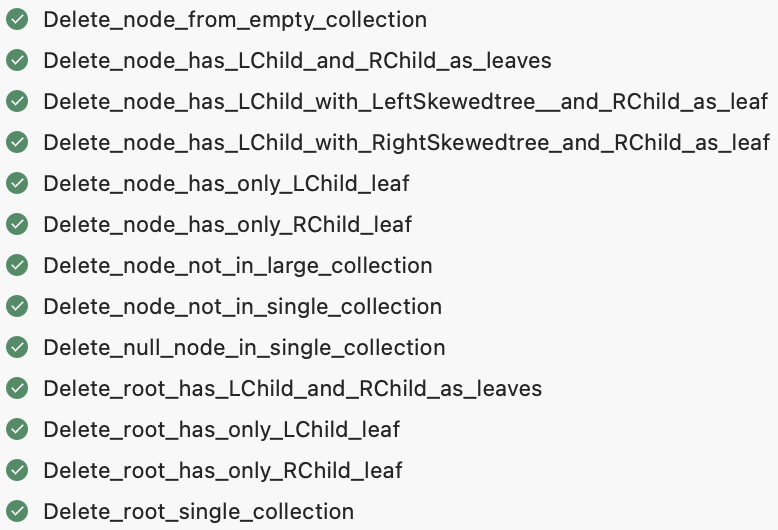
\includegraphics[height=6cm]{/Users/shridhar/Library/CloudStorage/OneDrive-QueenslandUniversityofTechnology/Bachelor of Mathematics and Information Technology/Year 4/CAB301 Algorithms/Assignment 2/Report/data/Summary-Delete.png}
\end{figure}

\subsubsection{Clear{()}}
The \codeword{Clear} method simply sets the root of a BST as null and the garbage collector for C\# in Visual Studio erases all other nodes from memory. Thus three tests were only needed. Testing involved clearing an empty array, clearing a \textit{single} collection and clearing a \textit{large} collection while checking if the \codeword{Number} property becomes 0 for each of them. 
\vspace{1mm}

\noindent
From the below summary it can be seen that all tests passed and the method performend as required. Test data, results and testing code can be found in the \hyperlink{subsubsection.5.3.6}{appendix for Clear}.
\vspace{2mm}

\noindent
\textbf{Unit testing summarisation}
\begin{figure}[H]
   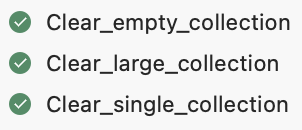
\includegraphics[height=1.8cm]{/Users/shridhar/Library/CloudStorage/OneDrive-QueenslandUniversityofTechnology/Bachelor of Mathematics and Information Technology/Year 4/CAB301 Algorithms/Assignment 2/Report/data/Summary-Clear.png}
\end{figure}

\subsubsection{NoDVDs}
This method simply outputted the sum of \codeword{TotalCopies} for each movie in the collection. Since \codeword{Insert} and \codeword{Delete} were already tested to perform as specified, there was no need to test \codeword{NoDVDs} before and after inserting or deleting. Hence it was simply tested for 3 static collections; an empty, \textit{single} and \textit{large} collection.
\vspace{1mm}

\noindent
From the below summary it can be seen that all tests passed and the method performend as required. Test data, results and testing code can be found in the \hyperlink{subsubsection.5.3.7}{appendix for Clear}.
\vspace{2mm}

\noindent
\textbf{Unit testing summarisation}
\begin{figure}[H]
   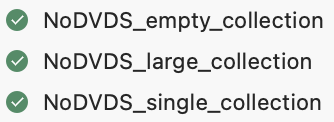
\includegraphics[height=1.6cm]{/Users/shridhar/Library/CloudStorage/OneDrive-QueenslandUniversityofTechnology/Bachelor of Mathematics and Information Technology/Year 4/CAB301 Algorithms/Assignment 2/Report/data/Summary-NoDVDs.png}
\end{figure}


\end{document}